\documentclass[11pt]{article}
\usepackage[margin=1in]{geometry}
\usepackage{amsmath,amssymb,amsthm}
\usepackage{hyperref}
\usepackage{enumitem}
\usepackage{graphicx}

\newtheorem{theorem}{Theorem}
\newtheorem{lemma}{Lemma}
\newtheorem{remark}{Remark}

\newcommand{\R}{\mathbb R}
\newcommand{\C}{\mathbb C}
\newcommand{\E}{\mathbb E}
\newcommand{\F}{\mathcal F}
\newcommand{\cS}{\mathcal S}
\newcommand{\dd}{\,d}
\newcommand{\supp}{\operatorname{supp}}

\title{A Combined Levy--Gaussian Fourier Multiplier Proof via General Weak Differential Subordination}
\author{Lane 19 packet for arXiv:1706.01731}
\date{June 20, 2026}

\begin{document}
\maketitle

\section*{Status}

This packet records a likely valid full solution to the concrete
multiplier-combination mechanism suggested on page 3 of Yaroslavtsev's paper
\cite{Yaroslavtsev2017Decompositions}.  The result gives a direct proof, using
the general weak differential subordination theorem from that paper, of the
mixed jump/continuous Fourier multiplier class stated in
\cite[Theorem 4.1]{Yaroslavtsev2017Multipliers}.  The obtained constant is the
general weak-differential-subordination constant
\[
        C_{p,X}:=\beta_{p,X}^2(\beta_{p,X}+1),
\]
not the sharper constant $\beta_{p,X}$ available from the special proof in
\cite{Yaroslavtsev2017Multipliers}.

This is not a claim to solve every open direction in
\cite{Yaroslavtsev2017Decompositions}.  The sharp continuous weak-subordination
constant problem and the broad stochastic-integral BDG problem for arbitrary
martingale noise remain separate.

\section*{Source Question}

The source paper says:

\begin{quote}
Alternative approaches to Fourier multipliers for functions with values in UMD
spaces have been constructed from the differential subordination for purely
discontinuous martingales [...] and for continuous martingales [...]. It
remains open whether one can combine these two approaches using the general
weak differential subordination theory.
\end{quote}

\begin{center}

\includegraphics[width=.92\linewidth]{figures/open_problem_crop.png}
\end{center}

\section*{The Concrete Result}

Let $V$ be a Levy measure on $\R^d$, let $\mu$ be a finite positive Borel
measure on $S^{d-1}$, and let $\phi$ and $\psi$ be scalar Borel functions with
$|\phi|\leq 1$ and $|\psi|\leq 1$.  Put
\[
 \Lambda(\xi)
 =
 \int_{\R^d}(1-\cos \xi\cdot z)\,V(dz)
 +\frac12\int_{S^{d-1}}(\xi\cdot\theta)^2\,\mu(d\theta),
\]
and define $m(\xi)=0$ when $\Lambda(\xi)=0$, while otherwise
\[
 m(\xi)=
 \frac{
 \int_{\R^d}(1-\cos \xi\cdot z)\phi(z)\,V(dz)
 +\frac12\int_{S^{d-1}}(\xi\cdot\theta)^2\psi(\theta)\,\mu(d\theta)}
 {\Lambda(\xi)}.
\]
This is the same mixed Levy/Gaussian symbol class appearing in
\cite[Theorem 4.1]{Yaroslavtsev2017Multipliers}; the relevant page is shown
below.

\begin{center}
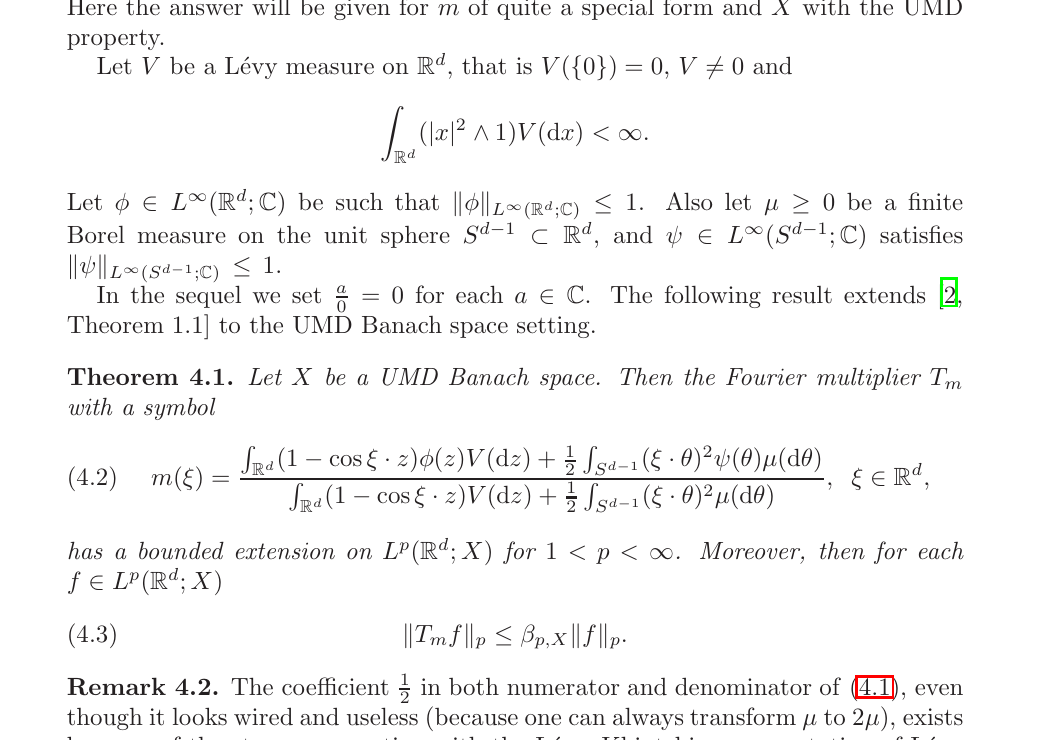
\includegraphics[width=.92\linewidth]{figures/supporting_mixed_multiplier_crop.png}
\end{center}

\begin{theorem}[combined WDS proof of the mixed multiplier bound]
Let $X$ be a real or complex UMD Banach space and $1<p<\infty$.  Then the
Fourier multiplier $T_m$, initially defined on
$\cS(\R^d)\otimes X$, extends to a bounded operator on $L^p(\R^d;X)$ and
\[
        \|T_m f\|_{L^p(\R^d;X)}
        \leq
        \beta_{p,X}^2(\beta_{p,X}+1)\,
        \|f\|_{L^p(\R^d;X)} .
\]
\end{theorem}

\section*{Proof Intuition}

The pure-jump proof uses a compound Poisson process and transforms each jump
increment by a scalar coefficient $\phi(z)$.  The continuous proof uses a
Brownian martingale and transforms each directional Brownian integrand by a
coefficient $\psi(\theta)$.  Put both noises in the same Levy process.  The
untransformed parabolic martingale has a continuous quadratic-variation part
and a jump quadratic-variation part.  The transformed martingale multiplies
the two corresponding pieces by contractions, so every scalar projection has
smaller quadratic variation.  Thus the transformed martingale is weakly
differentially subordinate to the original one.  The general theorem of
\cite{Yaroslavtsev2017Decompositions} applies once to this mixed martingale,
and the standard parabolic pairing computation gives exactly the quotient
symbol above.

\section*{Proof}

We give the proof first for a finite symmetric jump measure $\nu$ and finite
measure $\mu$, with bounded Borel coefficients.  The standard truncation and
symmetrization step at the end gives the stated Levy-measure formulation.

Let $L=(L_t)_{t\geq0}$ be the $\R^d$-valued Levy process whose characteristic
exponent is
\[
 \E e^{i\xi\cdot L_t}=e^{-t\Lambda(\xi)},\qquad
 \Lambda(\xi)=
 \int_{\R^d}(1-\cos \xi\cdot z)\,\nu(dz)
 +\frac12\int_{S^{d-1}}(\xi\cdot\theta)^2\,\mu(d\theta).
\]
Equivalently, $L=L^J+L^G$, where $L^J$ is a symmetric compound Poisson process
with jump intensity $\nu$, and
\[
        L^G_t=\int_{S^{d-1}}\theta\, W(d\theta,t)
\]
for an $L^2(S^{d-1},\mu)$-cylindrical Brownian motion $W$.  For
$s<t\leq0$ write $L_{s,t}=L_t-L_s$.  If $f\in C_c^\infty(\R^d;X)$, set
\[
        P_{t,0}f(x)=\E f(x+L_{t,0}),\qquad
        M_t=P_{t,0}f(x+L_{s,t}),\quad s\leq t\leq0.
\]
Then $M$ is the usual parabolic $X$-valued martingale and
$M_0=f(x+L_{s,0})$.

Define a transformed martingale $N$ by applying $\phi$ to jump increments and
$\psi$ to Brownian directional integrands:
\[
\begin{aligned}
N_t
&=
\int_s^t\int_{\R^d}
 \bigl(P_{r,0}f(x+L_{s,r-}+z)-P_{r,0}f(x+L_{s,r-})\bigr)
 \phi(z)\,\widetilde N^J(dr,dz)       \\
&\quad+
\int_s^t\int_{S^{d-1}}
 \partial_\theta P_{r,0}f(x+L_{s,r})\,\psi(\theta)\,
 W(d\theta,dr),
\end{aligned}
\]
where $\widetilde N^J$ is the compensated jump measure of $L^J$ and
$\partial_\theta$ denotes the directional derivative.  The corresponding
untransformed martingale differences are obtained by replacing
$\phi,\psi$ with $1$; their sum is $M_t-M_s$.

Fix a real continuous linear functional $x^*\in X^*$.  The quadratic variation
of $\langle N,x^*\rangle$ on $[s,t]$ is the sum of
\[
\int_s^t\int_{\R^d}
 \left|\left\langle
 P_{r,0}f(x+L_{s,r-}+z)-P_{r,0}f(x+L_{s,r-}),x^*
 \right\rangle\right|^2
 |\phi(z)|^2\,N^J(dr,dz)
\]
and
\[
\int_s^t\int_{S^{d-1}}
 \left|\left\langle \partial_\theta P_{r,0}f(x+L_{s,r}),x^*\right\rangle\right|^2
 |\psi(\theta)|^2\,\mu(d\theta)\,dr .
\]
Since $|\phi|\leq1$ and $|\psi|\leq1$, this is bounded by the corresponding
quadratic variation of $\langle M,x^*\rangle$.  Also $N_s=0$, while
$|\langle N_s,x^*\rangle|\leq |\langle M_s,x^*\rangle|$.  Hence $N$
is weakly differentially subordinate to $M$.  Yaroslavtsev's general weak
differential subordination theorem \cite[Theorem 4.1]{Yaroslavtsev2017Decompositions}
therefore gives
\[
 \bigl(\E\|N_0\|^p\bigr)^{1/p}
 \leq C_{p,X}\bigl(\E\|M_0\|^p\bigr)^{1/p}.
\]
After integration in $x$ and translation invariance,
\[
 \int_{\R^d}\E\|N_0(x;s,0;f)\|^p\,dx
 \leq C_{p,X}^p\|f\|_{L^p(\R^d;X)}^p .
\]

Pair $N_0(x;s,0;f)$ against a test function
$g(x+L_{s,0})$, integrate in $x$, and use the Ito isometry/compensation
identities for the jump and Brownian parts.  The same calculation as in the
Ba\~nuelos--Bogdan parabolic proof gives
\[
 \int_{\R^d}\E\langle N_0(x;s,0;f),g(x+L_{s,0})\rangle\,dx
 =
 \int_{\R^d}\langle T_{m_s}f(x),g(x)\rangle\,dx,
\]
where
\[
 m_s(\xi)
 =
 \bigl(1-e^{-2|s|\Lambda(\xi)}\bigr)\,
 \frac{
 \int_{\R^d}(1-\cos \xi\cdot z)\phi(z)\,\nu(dz)
 +\frac12\int_{S^{d-1}}(\xi\cdot\theta)^2\psi(\theta)\,\mu(d\theta)}
 {\Lambda(\xi)}
\]
with the value $0$ on $\{\Lambda=0\}$.  Indeed, each jump or Brownian
contribution at time $r$ contributes one factor $e^{-(0-r)\Lambda(\xi)}$ from
the parabolic extension and another from the terminal test function; integrating
over $r\in[s,0]$ yields the factor $1-e^{-2|s|\Lambda(\xi)}$ divided by the
denominator.  H\"older duality then gives
\[
        \|T_{m_s}f\|_{L^p(\R^d;X)}
        \leq C_{p,X}\|f\|_{L^p(\R^d;X)} .
\]
Letting $s\to-\infty$, $m_s(\xi)\to m(\xi)$ pointwise.  For
$f\in C_c^\infty(\R^d;X)$, Plancherel on finite-dimensional ranges gives
$T_{m_s}f\to T_mf$ in $L^2$, and Fatou gives the same $L^p$ bound for $T_mf$.
Density extends $T_m$ to all of $L^p(\R^d;X)$.

For a general Levy measure $V$, set
$V_n=1_{\{1/n\leq |z|\leq n\}}V$ and apply the finite-measure result to $V_n$.
The integrability condition
$\int(|z|^2\wedge1)\,V(dz)<\infty$ and dominated convergence imply pointwise
convergence of the corresponding symbols.  If $V$ or $\mu$ is not symmetric,
replace it by its symmetrization and replace the coefficient by the associated
Radon--Nikodym average; since $1-\cos(\xi\cdot z)$ and
$(\xi\cdot\theta)^2$ are even, this leaves the symbol unchanged and preserves
the bound $|\phi|,|\psi|\leq1$.  This proves the theorem.

For complex $X$ and complex coefficients, apply the argument to the realification
of $X$.  Multiplication by a scalar of modulus at most one is a real-linear
contraction, so the weak-subordination check above is unchanged.
\qed

\section*{Verification Notes and Limitations}

\begin{itemize}[leftmargin=2em]
\item The proof uses only the general weak differential subordination theorem
from \cite{Yaroslavtsev2017Decompositions} and the standard
Ba\~nuelos--Bogdan parabolic multiplier computation.
\item The result is full for the selected concrete source route: it verifies
the combination mechanism for the canonical mixed Levy/Gaussian symbol class.
It does not claim a new class of multipliers beyond the earlier Theorem 4.1 of
\cite{Yaroslavtsev2017Multipliers}.
\item The constant is deliberately not sharp.  The direct general-WDS route
inherits $C_{p,X}=\beta_{p,X}^2(\beta_{p,X}+1)$, whereas the special proof in
\cite{Yaroslavtsev2017Multipliers} gives $\beta_{p,X}$.
\item Novelty search: local indexes were searched for arXiv:1706.01731, the
open sentence, weak differential subordination, Fourier multipliers, and the
nearby arXiv ids 1703.07817 and 1805.03948.  Web exact-phrase searches for the
open sentence and for a combined WDS multiplier proof did not find a later
explicit answer.
\end{itemize}

\section*{Human Review Recommendation}

Review the multiplier-symbol computation in the mixed parabolic pairing,
especially the factor $1-e^{-2|s|\Lambda(\xi)}$ and the symmetrization step for
non-symmetric measures.  The weak differential subordination step itself is
straightforward and is the intended new mechanism of the packet.

\begin{thebibliography}{9}

\bibitem{Yaroslavtsev2017Decompositions}
I. S. Yaroslavtsev.
\newblock Martingale decompositions and weak differential subordination in UMD Banach spaces.
\newblock arXiv:1706.01731, 2017.

\bibitem{Yaroslavtsev2017Multipliers}
I. S. Yaroslavtsev.
\newblock Fourier multipliers and weak differential subordination of martingales in UMD Banach spaces.
\newblock arXiv:1703.07817, 2017.

\bibitem{BanuelosBogdan}
R. Ba\~nuelos and K. Bogdan.
\newblock Levy processes and Fourier multipliers.
\newblock \emph{J. Funct. Anal.} 250(1):197--213, 2007.

\bibitem{BBB}
R. Ba\~nuelos, A. Bielaszewski, and K. Bogdan.
\newblock Fourier multipliers for non-symmetric Levy processes.
\newblock In \emph{Marcinkiewicz centenary volume}, Banach Center Publ. 95, 9--25, 2011.

\end{thebibliography}

\end{document}
